% Generated by Sphinx.
\def\sphinxdocclass{report}
\documentclass[letterpaper,10pt]{sphinxmanual}
\usepackage[utf8]{inputenc}
\DeclareUnicodeCharacter{00A0}{\nobreakspace}
\usepackage[T1]{fontenc}
\usepackage{babel}
\usepackage{times}
\usepackage[Sonny]{fncychap}
\usepackage{longtable}
\usepackage{sphinx}
\usepackage{multirow}


\title{GPTwoSample Documentation}
\date{April 07, 2013}
\release{0.1.7a}
\author{Oliver Stegle, Max Zwießele}
\newcommand{\sphinxlogo}{}
\renewcommand{\releasename}{Release}
\makeindex

\makeatletter
\def\PYG@reset{\let\PYG@it=\relax \let\PYG@bf=\relax%
    \let\PYG@ul=\relax \let\PYG@tc=\relax%
    \let\PYG@bc=\relax \let\PYG@ff=\relax}
\def\PYG@tok#1{\csname PYG@tok@#1\endcsname}
\def\PYG@toks#1+{\ifx\relax#1\empty\else%
    \PYG@tok{#1}\expandafter\PYG@toks\fi}
\def\PYG@do#1{\PYG@bc{\PYG@tc{\PYG@ul{%
    \PYG@it{\PYG@bf{\PYG@ff{#1}}}}}}}
\def\PYG#1#2{\PYG@reset\PYG@toks#1+\relax+\PYG@do{#2}}

\expandafter\def\csname PYG@tok@gd\endcsname{\def\PYG@tc##1{\textcolor[rgb]{0.63,0.00,0.00}{##1}}}
\expandafter\def\csname PYG@tok@gu\endcsname{\let\PYG@bf=\textbf\def\PYG@tc##1{\textcolor[rgb]{0.50,0.00,0.50}{##1}}}
\expandafter\def\csname PYG@tok@gt\endcsname{\def\PYG@tc##1{\textcolor[rgb]{0.00,0.25,0.82}{##1}}}
\expandafter\def\csname PYG@tok@gs\endcsname{\let\PYG@bf=\textbf}
\expandafter\def\csname PYG@tok@gr\endcsname{\def\PYG@tc##1{\textcolor[rgb]{1.00,0.00,0.00}{##1}}}
\expandafter\def\csname PYG@tok@cm\endcsname{\let\PYG@it=\textit\def\PYG@tc##1{\textcolor[rgb]{0.25,0.50,0.56}{##1}}}
\expandafter\def\csname PYG@tok@vg\endcsname{\def\PYG@tc##1{\textcolor[rgb]{0.73,0.38,0.84}{##1}}}
\expandafter\def\csname PYG@tok@m\endcsname{\def\PYG@tc##1{\textcolor[rgb]{0.13,0.50,0.31}{##1}}}
\expandafter\def\csname PYG@tok@mh\endcsname{\def\PYG@tc##1{\textcolor[rgb]{0.13,0.50,0.31}{##1}}}
\expandafter\def\csname PYG@tok@cs\endcsname{\def\PYG@tc##1{\textcolor[rgb]{0.25,0.50,0.56}{##1}}\def\PYG@bc##1{\setlength{\fboxsep}{0pt}\colorbox[rgb]{1.00,0.94,0.94}{\strut ##1}}}
\expandafter\def\csname PYG@tok@ge\endcsname{\let\PYG@it=\textit}
\expandafter\def\csname PYG@tok@vc\endcsname{\def\PYG@tc##1{\textcolor[rgb]{0.73,0.38,0.84}{##1}}}
\expandafter\def\csname PYG@tok@il\endcsname{\def\PYG@tc##1{\textcolor[rgb]{0.13,0.50,0.31}{##1}}}
\expandafter\def\csname PYG@tok@go\endcsname{\def\PYG@tc##1{\textcolor[rgb]{0.19,0.19,0.19}{##1}}}
\expandafter\def\csname PYG@tok@cp\endcsname{\def\PYG@tc##1{\textcolor[rgb]{0.00,0.44,0.13}{##1}}}
\expandafter\def\csname PYG@tok@gi\endcsname{\def\PYG@tc##1{\textcolor[rgb]{0.00,0.63,0.00}{##1}}}
\expandafter\def\csname PYG@tok@gh\endcsname{\let\PYG@bf=\textbf\def\PYG@tc##1{\textcolor[rgb]{0.00,0.00,0.50}{##1}}}
\expandafter\def\csname PYG@tok@ni\endcsname{\let\PYG@bf=\textbf\def\PYG@tc##1{\textcolor[rgb]{0.84,0.33,0.22}{##1}}}
\expandafter\def\csname PYG@tok@nl\endcsname{\let\PYG@bf=\textbf\def\PYG@tc##1{\textcolor[rgb]{0.00,0.13,0.44}{##1}}}
\expandafter\def\csname PYG@tok@nn\endcsname{\let\PYG@bf=\textbf\def\PYG@tc##1{\textcolor[rgb]{0.05,0.52,0.71}{##1}}}
\expandafter\def\csname PYG@tok@no\endcsname{\def\PYG@tc##1{\textcolor[rgb]{0.38,0.68,0.84}{##1}}}
\expandafter\def\csname PYG@tok@na\endcsname{\def\PYG@tc##1{\textcolor[rgb]{0.25,0.44,0.63}{##1}}}
\expandafter\def\csname PYG@tok@nb\endcsname{\def\PYG@tc##1{\textcolor[rgb]{0.00,0.44,0.13}{##1}}}
\expandafter\def\csname PYG@tok@nc\endcsname{\let\PYG@bf=\textbf\def\PYG@tc##1{\textcolor[rgb]{0.05,0.52,0.71}{##1}}}
\expandafter\def\csname PYG@tok@nd\endcsname{\let\PYG@bf=\textbf\def\PYG@tc##1{\textcolor[rgb]{0.33,0.33,0.33}{##1}}}
\expandafter\def\csname PYG@tok@ne\endcsname{\def\PYG@tc##1{\textcolor[rgb]{0.00,0.44,0.13}{##1}}}
\expandafter\def\csname PYG@tok@nf\endcsname{\def\PYG@tc##1{\textcolor[rgb]{0.02,0.16,0.49}{##1}}}
\expandafter\def\csname PYG@tok@si\endcsname{\let\PYG@it=\textit\def\PYG@tc##1{\textcolor[rgb]{0.44,0.63,0.82}{##1}}}
\expandafter\def\csname PYG@tok@s2\endcsname{\def\PYG@tc##1{\textcolor[rgb]{0.25,0.44,0.63}{##1}}}
\expandafter\def\csname PYG@tok@vi\endcsname{\def\PYG@tc##1{\textcolor[rgb]{0.73,0.38,0.84}{##1}}}
\expandafter\def\csname PYG@tok@nt\endcsname{\let\PYG@bf=\textbf\def\PYG@tc##1{\textcolor[rgb]{0.02,0.16,0.45}{##1}}}
\expandafter\def\csname PYG@tok@nv\endcsname{\def\PYG@tc##1{\textcolor[rgb]{0.73,0.38,0.84}{##1}}}
\expandafter\def\csname PYG@tok@s1\endcsname{\def\PYG@tc##1{\textcolor[rgb]{0.25,0.44,0.63}{##1}}}
\expandafter\def\csname PYG@tok@gp\endcsname{\let\PYG@bf=\textbf\def\PYG@tc##1{\textcolor[rgb]{0.78,0.36,0.04}{##1}}}
\expandafter\def\csname PYG@tok@sh\endcsname{\def\PYG@tc##1{\textcolor[rgb]{0.25,0.44,0.63}{##1}}}
\expandafter\def\csname PYG@tok@ow\endcsname{\let\PYG@bf=\textbf\def\PYG@tc##1{\textcolor[rgb]{0.00,0.44,0.13}{##1}}}
\expandafter\def\csname PYG@tok@sx\endcsname{\def\PYG@tc##1{\textcolor[rgb]{0.78,0.36,0.04}{##1}}}
\expandafter\def\csname PYG@tok@bp\endcsname{\def\PYG@tc##1{\textcolor[rgb]{0.00,0.44,0.13}{##1}}}
\expandafter\def\csname PYG@tok@c1\endcsname{\let\PYG@it=\textit\def\PYG@tc##1{\textcolor[rgb]{0.25,0.50,0.56}{##1}}}
\expandafter\def\csname PYG@tok@kc\endcsname{\let\PYG@bf=\textbf\def\PYG@tc##1{\textcolor[rgb]{0.00,0.44,0.13}{##1}}}
\expandafter\def\csname PYG@tok@c\endcsname{\let\PYG@it=\textit\def\PYG@tc##1{\textcolor[rgb]{0.25,0.50,0.56}{##1}}}
\expandafter\def\csname PYG@tok@mf\endcsname{\def\PYG@tc##1{\textcolor[rgb]{0.13,0.50,0.31}{##1}}}
\expandafter\def\csname PYG@tok@err\endcsname{\def\PYG@bc##1{\setlength{\fboxsep}{0pt}\fcolorbox[rgb]{1.00,0.00,0.00}{1,1,1}{\strut ##1}}}
\expandafter\def\csname PYG@tok@kd\endcsname{\let\PYG@bf=\textbf\def\PYG@tc##1{\textcolor[rgb]{0.00,0.44,0.13}{##1}}}
\expandafter\def\csname PYG@tok@ss\endcsname{\def\PYG@tc##1{\textcolor[rgb]{0.32,0.47,0.09}{##1}}}
\expandafter\def\csname PYG@tok@sr\endcsname{\def\PYG@tc##1{\textcolor[rgb]{0.14,0.33,0.53}{##1}}}
\expandafter\def\csname PYG@tok@mo\endcsname{\def\PYG@tc##1{\textcolor[rgb]{0.13,0.50,0.31}{##1}}}
\expandafter\def\csname PYG@tok@mi\endcsname{\def\PYG@tc##1{\textcolor[rgb]{0.13,0.50,0.31}{##1}}}
\expandafter\def\csname PYG@tok@kn\endcsname{\let\PYG@bf=\textbf\def\PYG@tc##1{\textcolor[rgb]{0.00,0.44,0.13}{##1}}}
\expandafter\def\csname PYG@tok@o\endcsname{\def\PYG@tc##1{\textcolor[rgb]{0.40,0.40,0.40}{##1}}}
\expandafter\def\csname PYG@tok@kr\endcsname{\let\PYG@bf=\textbf\def\PYG@tc##1{\textcolor[rgb]{0.00,0.44,0.13}{##1}}}
\expandafter\def\csname PYG@tok@s\endcsname{\def\PYG@tc##1{\textcolor[rgb]{0.25,0.44,0.63}{##1}}}
\expandafter\def\csname PYG@tok@kp\endcsname{\def\PYG@tc##1{\textcolor[rgb]{0.00,0.44,0.13}{##1}}}
\expandafter\def\csname PYG@tok@w\endcsname{\def\PYG@tc##1{\textcolor[rgb]{0.73,0.73,0.73}{##1}}}
\expandafter\def\csname PYG@tok@kt\endcsname{\def\PYG@tc##1{\textcolor[rgb]{0.56,0.13,0.00}{##1}}}
\expandafter\def\csname PYG@tok@sc\endcsname{\def\PYG@tc##1{\textcolor[rgb]{0.25,0.44,0.63}{##1}}}
\expandafter\def\csname PYG@tok@sb\endcsname{\def\PYG@tc##1{\textcolor[rgb]{0.25,0.44,0.63}{##1}}}
\expandafter\def\csname PYG@tok@k\endcsname{\let\PYG@bf=\textbf\def\PYG@tc##1{\textcolor[rgb]{0.00,0.44,0.13}{##1}}}
\expandafter\def\csname PYG@tok@se\endcsname{\let\PYG@bf=\textbf\def\PYG@tc##1{\textcolor[rgb]{0.25,0.44,0.63}{##1}}}
\expandafter\def\csname PYG@tok@sd\endcsname{\let\PYG@it=\textit\def\PYG@tc##1{\textcolor[rgb]{0.25,0.44,0.63}{##1}}}

\def\PYGZbs{\char`\\}
\def\PYGZus{\char`\_}
\def\PYGZob{\char`\{}
\def\PYGZcb{\char`\}}
\def\PYGZca{\char`\^}
\def\PYGZam{\char`\&}
\def\PYGZlt{\char`\<}
\def\PYGZgt{\char`\>}
\def\PYGZsh{\char`\#}
\def\PYGZpc{\char`\%}
\def\PYGZdl{\char`\$}
\def\PYGZti{\char`\~}
% for compatibility with earlier versions
\def\PYGZat{@}
\def\PYGZlb{[}
\def\PYGZrb{]}
\makeatother

\begin{document}

\maketitle
\tableofcontents
\phantomsection\label{index::doc}


This package provides Gaussian Process based differential gene
expression detection.

Contents:
\phantomsection\label{base:module-gptwosample}\index{gptwosample (module)}

\chapter{Package for using GPTwoSample}
\label{base:package-for-using-gptwosample}\label{base::doc}\label{base:welcome-to-gptwosample}
This module allows the user to compare two timelines with respect to diffferential expression.

It compares two timeseries against each other, depicting whether these two
timeseries were more likely drawn from the same function, or from
different ones. This prediction is defined by which covariance function \code{pygp.covar} you use.

Created on Jun 15, 2011

@author: Max Zwiessele, Oliver Stegle
\index{TwoSample (class in gptwosample.twosample.twosample)}

\begin{fulllineitems}
\phantomsection\label{base:gptwosample.twosample.twosample.TwoSample}\pysiglinewithargsret{\strong{class }\code{gptwosample.twosample.twosample.}\bfcode{TwoSample}}{\emph{T}, \emph{Y}, \emph{covar\_common=None}, \emph{covar\_individual\_1=None}, \emph{covar\_individual\_2=None}}{}
Bases: \code{object}

Run GPTwoSample on given data.
\begin{description}
\item[{\textbf{Parameters}:}] \leavevmode\begin{itemize}
\item {} 
T : TimePoints {[}n x r x t{]}    {[}Samples x Replicates x Timepoints{]}

\item {} 
Y : ExpressionMatrix {[}n x r x t x d{]}      {[}Samples x Replicates x Timepoints x Genes{]}

\end{itemize}

\item[{\textbf{Fields}:}] \leavevmode\begin{itemize}
\item {} 
T: Time Points {[}n x r x t{]} {[}Samples x Replicates x Timepoints{]}

\item {} 
Y: Expression {[}n x r x t x d{]} {[}Samples x Replicates x Timepoints x Genes{]}

\item {} 
X: Confounders {[}nrt x 1+q{]} {[}SamplesReplicatesTimepoints x T+q{]}

\item {} 
lvm\_covariance: GPLVM covaraince function used for confounder learning

\item {} 
n: Samples

\item {} 
r: Replicates

\item {} 
t: Timepoints

\item {} 
d: Genes

\item {} 
q: Confounder Components

\end{itemize}

\end{description}
\index{bayes\_factors() (gptwosample.twosample.twosample.TwoSample method)}

\begin{fulllineitems}
\phantomsection\label{base:gptwosample.twosample.twosample.TwoSample.bayes_factors}\pysiglinewithargsret{\bfcode{bayes\_factors}}{\emph{likelihoods=None}}{}
get list of bayes\_factors for all genes.
\begin{description}
\item[{\textbf{returns}:}] \leavevmode
bayes\_factor for each gene in Y

\end{description}

\end{fulllineitems}

\index{plot() (gptwosample.twosample.twosample.TwoSample method)}

\begin{fulllineitems}
\phantomsection\label{base:gptwosample.twosample.twosample.TwoSample.plot}\pysiglinewithargsret{\bfcode{plot}}{\emph{xlabel='input'}, \emph{ylabel='ouput'}, \emph{title=None}, \emph{interval\_indices=None}, \emph{alpha=None}, \emph{legend=True}, \emph{replicate\_indices=None}, \emph{shift=None}, \emph{timeshift=False}, \emph{*args}, \emph{**kwargs}}{}
iterate through all genes and plot

\end{fulllineitems}

\index{predict\_likelihoods() (gptwosample.twosample.twosample.TwoSample method)}

\begin{fulllineitems}
\phantomsection\label{base:gptwosample.twosample.twosample.TwoSample.predict_likelihoods}\pysiglinewithargsret{\bfcode{predict\_likelihoods}}{\emph{T}, \emph{Y}, \emph{message='Predicting Likelihoods: `}, \emph{messages=False}, \emph{priors=None}, \emph{**kwargs}}{}
Predict all likelihoods for all genes, given in Y

\textbf{parameters}:
\begin{quote}
\begin{description}
\item[{indices}] \leavevmode{[}{[}int{]}{]}
list (or array-like) for gene indices to predict, if None all genes will be predicted

\item[{message: str}] \leavevmode
printing message

\item[{kwargs: \{...\}}] \leavevmode
kwargs for \code{gptwosample.twosample.GPTwoSampleBase.predict\_model\_likelihoods()}

\end{description}
\end{quote}

\end{fulllineitems}

\index{predict\_means\_variances() (gptwosample.twosample.twosample.TwoSample method)}

\begin{fulllineitems}
\phantomsection\label{base:gptwosample.twosample.twosample.TwoSample.predict_means_variances}\pysiglinewithargsret{\bfcode{predict\_means\_variances}}{\emph{interpolation\_interval}, \emph{indices=None}, \emph{message='Predicting means and variances: `}, \emph{*args}, \emph{**kwargs}}{}
Predicts means and variances for all genes given in Y for given interpolation\_interval

\end{fulllineitems}

\index{set\_data() (gptwosample.twosample.twosample.TwoSample method)}

\begin{fulllineitems}
\phantomsection\label{base:gptwosample.twosample.twosample.TwoSample.set_data}\pysiglinewithargsret{\bfcode{set\_data}}{\emph{T}, \emph{Y}}{}
Set data by time T and expression matrix Y:

\textbf{Parameters}:
\begin{quote}
\begin{description}
\item[{T}] \leavevmode{[}real {[}n x r x t{]}{]}
All Timepoints with shape {[}Samples x Replicates x Timepoints{]}

\item[{Y}] \leavevmode{[}real {[}n x r x t x d{]}{]}
All expression values given in the form: {[}Samples x Replicates x Timepoints x Genes{]}

\end{description}
\end{quote}

\end{fulllineitems}


\end{fulllineitems}

\index{TwoSampleConfounder (class in gptwosample.confounder.confounder)}

\begin{fulllineitems}
\phantomsection\label{base:gptwosample.confounder.confounder.TwoSampleConfounder}\pysiglinewithargsret{\strong{class }\code{gptwosample.confounder.confounder.}\bfcode{TwoSampleConfounder}}{\emph{T}, \emph{Y}, \emph{q=4}, \emph{lvm\_covariance=None}, \emph{init='random'}, \emph{covar\_common=None}, \emph{covar\_individual\_1=None}, \emph{covar\_individual\_2=None}}{}
Bases: {\hyperref[base:gptwosample.twosample.twosample.TwoSample]{\code{gptwosample.twosample.twosample.TwoSample}}}

Run GPTwoSample on given Data
\begin{description}
\item[{\textbf{Parameters}:}] \leavevmode\begin{itemize}
\item {} 
T : TimePoints {[}n x r x t{]}    {[}Samples x Replicates x Timepoints{]}

\item {} 
Y : ExpressionMatrix {[}n x r x t x d{]}      {[}Samples x Replicates x Timepoints x Genes{]}

\item {} 
q : Number of Confounders to use

\item {} 
lvm\_covariance : optional - set covariance to use in confounder learning

\item {} 
init : {[}random, pca{]}

\end{itemize}

\item[{\textbf{Fields}:}] \leavevmode\begin{itemize}
\item {} 
T: Time Points {[}n x r x t{]} {[}Samples x Replicates x Timepoints{]}

\item {} 
Y: Expression {[}n x r x t x d{]} {[}Samples x Replicates x Timepoints x Genes{]}

\item {} 
X: Confounders {[}nrt x 1+q{]} {[}SamplesReplicatesTimepoints x T+q{]}

\item {} 
lvm\_covariance: GPLVM covaraince function used for confounder learning

\item {} 
n: Samples

\item {} 
r: Replicates

\item {} 
t: Timepoints

\item {} 
d: Genes

\item {} 
q: Confounder Components

\end{itemize}

\end{description}
\index{initialize\_twosample\_covariance() (gptwosample.confounder.confounder.TwoSampleConfounder method)}

\begin{fulllineitems}
\phantomsection\label{base:gptwosample.confounder.confounder.TwoSampleConfounder.initialize_twosample_covariance}\pysiglinewithargsret{\bfcode{initialize\_twosample\_covariance}}{\emph{covar\_common=\textless{}function \textless{}lambda\textgreater{} at 0x112fd77d0\textgreater{}}, \emph{covar\_individual\_1=\textless{}function \textless{}lambda\textgreater{} at 0x112fd76e0\textgreater{}}, \emph{covar\_individual\_2=\textless{}function \textless{}lambda\textgreater{} at 0x112fd7f50\textgreater{}}}{}
initialize twosample covariance with function covariance(XX), where XX
is a FixedCF with the learned confounder matrix.

default is SumCF({[}SqexpCFARD(1), FixedCF(self.K\_conf.copy()), BiasCF(){]})

\end{fulllineitems}

\index{learn\_confounder\_matrix() (gptwosample.confounder.confounder.TwoSampleConfounder method)}

\begin{fulllineitems}
\phantomsection\label{base:gptwosample.confounder.confounder.TwoSampleConfounder.learn_confounder_matrix}\pysiglinewithargsret{\bfcode{learn\_confounder\_matrix}}{\emph{ard\_indices=None}, \emph{x=None}, \emph{messages=True}, \emph{gradient\_tolerance=1e-12}, \emph{lvm\_dimension\_indices=None}, \emph{gradcheck=False}, \emph{maxiter=10000}}{}
Learn confounder matrix with this model.

\textbf{Parameters}:
\begin{quote}
\begin{description}
\item[{x}] \leavevmode{[}array-like{]}
If you provided an own lvm\_covariance you have to specify
the X to use within GPLVM

\item[{lvm\_dimension\_indices}] \leavevmode{[}{[}int{]}{]}
If you specified an own lvm\_covariance you have to specify
the dimension indices for GPLVM

\item[{ard\_indices}] \leavevmode{[}{[}indices{]}{]}
If you provided an own lvm\_covariance, give the ard indices of the covariance here,
to be able to use the correct hyperparameters for calculating the confounder covariance matrix.

\end{description}
\end{quote}

\end{fulllineitems}


\end{fulllineitems}

\index{TwoSampleShare (class in gptwosample.twosample.twosample\_base)}

\begin{fulllineitems}
\phantomsection\label{base:gptwosample.twosample.twosample_base.TwoSampleShare}\pysiglinewithargsret{\strong{class }\code{gptwosample.twosample.twosample\_base.}\bfcode{TwoSampleShare}}{\emph{covar}, \emph{*args}, \emph{**kwargs}}{}
Bases: {\hyperref[base:gptwosample.twosample.twosample_base.TwoSampleBase]{\code{gptwosample.twosample.twosample\_base.TwoSampleBase}}}

This class provides comparison of two Timeline Groups to each other.

see {\hyperref[base:gptwosample.twosample.twosample_base.TwoSampleBase]{\code{gptwosample.twosample.twosample\_base.TwoSampleBase}}} for detailed description of provided methods.

\end{fulllineitems}

\index{TwoSampleSeparate (class in gptwosample.twosample.twosample\_base)}

\begin{fulllineitems}
\phantomsection\label{base:gptwosample.twosample.twosample_base.TwoSampleSeparate}\pysiglinewithargsret{\strong{class }\code{gptwosample.twosample.twosample\_base.}\bfcode{TwoSampleSeparate}}{\emph{covar\_individual\_1}, \emph{covar\_individual\_2}, \emph{covar\_common}, \emph{**kwargs}}{}
Bases: {\hyperref[base:gptwosample.twosample.twosample_base.TwoSampleBase]{\code{gptwosample.twosample.twosample\_base.TwoSampleBase}}}

This class provides comparison of two Timeline Groups to one another, inlcuding timeshifts in replicates, respectively.

see {\hyperref[base:gptwosample.twosample.twosample_base.TwoSampleBase]{\code{gptwosample.twosample.twosample\_base.TwoSampleBase}}} for detailed description of provided methods.

Note that this model will need one covariance function for each model, respectively!

\end{fulllineitems}

\index{TwoSampleBase (class in gptwosample.twosample.twosample\_base)}

\begin{fulllineitems}
\phantomsection\label{base:gptwosample.twosample.twosample_base.TwoSampleBase}\pysiglinewithargsret{\strong{class }\code{gptwosample.twosample.twosample\_base.}\bfcode{TwoSampleBase}}{\emph{learn\_hyperparameters=True}, \emph{priors=None}, \emph{initial\_hyperparameters=None}, \emph{**kwargs}}{}
Bases: \code{object}

TwoSampleBase object with the given covariance function covar.
\index{bayes\_factor() (gptwosample.twosample.twosample\_base.TwoSampleBase method)}

\begin{fulllineitems}
\phantomsection\label{base:gptwosample.twosample.twosample_base.TwoSampleBase.bayes_factor}\pysiglinewithargsret{\bfcode{bayes\_factor}}{\emph{model\_likelihoods=None}}{}
Return the Bayes Factor for the given log marginal likelihoods model\_likelihoods

\textbf{Parameters:}
\begin{description}
\item[{model\_likelihoods}] \leavevmode{[}\{`individual': \emph{the individual likelihoods}, `common': \emph{the common likelihoods}\}{]}
The likelihoods calculated by
predict\_model\_likelihoods(training\_data)
for given training data training\_data.

\end{description}

\end{fulllineitems}

\index{get\_data() (gptwosample.twosample.twosample\_base.TwoSampleBase method)}

\begin{fulllineitems}
\phantomsection\label{base:gptwosample.twosample.twosample_base.TwoSampleBase.get_data}\pysiglinewithargsret{\bfcode{get\_data}}{\emph{model='common'}, \emph{index=None}}{}
get inputs of model \emph{model} with group index \emph{index}.
If index is None, the whole model group will be returned.

\end{fulllineitems}

\index{get\_learned\_hyperparameters() (gptwosample.twosample.twosample\_base.TwoSampleBase method)}

\begin{fulllineitems}
\phantomsection\label{base:gptwosample.twosample.twosample_base.TwoSampleBase.get_learned_hyperparameters}\pysiglinewithargsret{\bfcode{get\_learned\_hyperparameters}}{}{}
Returns learned hyperparameters in model structure, if already learned.

\end{fulllineitems}

\index{get\_model\_likelihoods() (gptwosample.twosample.twosample\_base.TwoSampleBase method)}

\begin{fulllineitems}
\phantomsection\label{base:gptwosample.twosample.twosample_base.TwoSampleBase.get_model_likelihoods}\pysiglinewithargsret{\bfcode{get\_model\_likelihoods}}{}{}
Returns all calculated likelihoods in model structure. If not calculated returns None in model structure.

\end{fulllineitems}

\index{get\_predicted\_mean\_variance() (gptwosample.twosample.twosample\_base.TwoSampleBase method)}

\begin{fulllineitems}
\phantomsection\label{base:gptwosample.twosample.twosample_base.TwoSampleBase.get_predicted_mean_variance}\pysiglinewithargsret{\bfcode{get\_predicted\_mean\_variance}}{}{}
Get the predicted mean and variance as:

\begin{Verbatim}[commandchars=\\\{\}]
\PYGZob{}'individual':\PYGZob{}'mean':[pointwise mean], 'var':[pointwise variance]\PYGZcb{},
     'common':\PYGZob{}'mean':[pointwise mean], 'var':[pointwise variance]\PYGZcb{}\PYGZcb{}
\end{Verbatim}

If not yet predicted it will return `individual' and `common' empty.

\end{fulllineitems}

\index{plot() (gptwosample.twosample.twosample\_base.TwoSampleBase method)}

\begin{fulllineitems}
\phantomsection\label{base:gptwosample.twosample.twosample_base.TwoSampleBase.plot}\pysiglinewithargsret{\bfcode{plot}}{\emph{xlabel='input'}, \emph{ylabel='ouput'}, \emph{title=None}, \emph{interval\_indices=None}, \emph{alpha=None}, \emph{legend=True}, \emph{replicate\_indices=None}, \emph{shift=None}, \emph{*args}, \emph{**kwargs}}{}
Plot the results given by last prediction.

Two Instance Plots of comparing two groups to each other:

\textbf{Parameters:}
\begin{description}
\item[{twosample\_object}] \leavevmode{[}\code{gptwosample.twosample}{]}
GPTwoSample object, on which already `predict' was called.

\end{description}

\textbf{Differential Groups:}

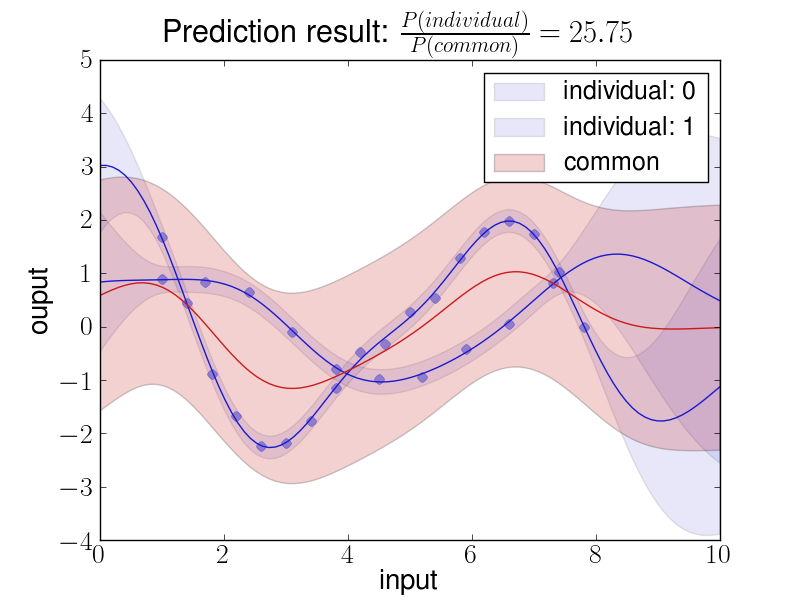
\includegraphics[height=8cm]{plotGPTwoSampleDifferential.png}

\textbf{Non-Differential Groups:}

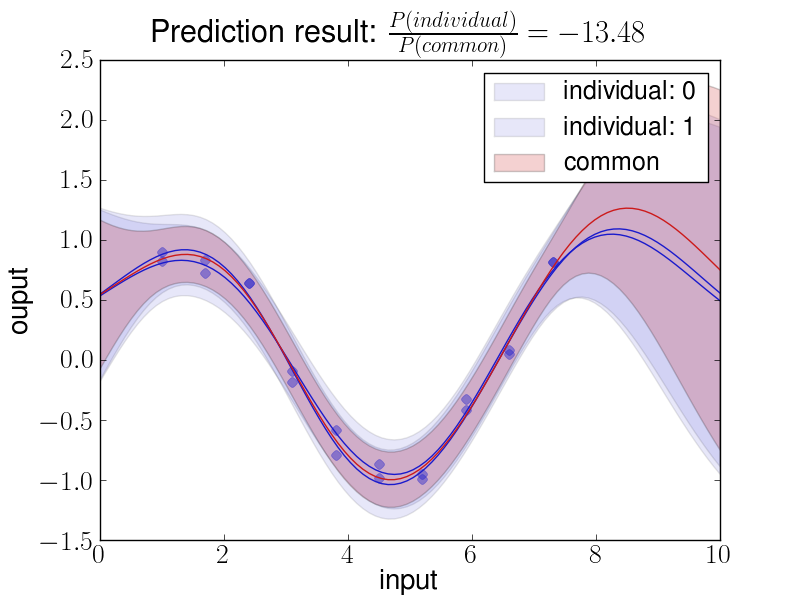
\includegraphics[height=8cm]{plotGPTwoSampleSame.png}
\begin{description}
\item[{Returns:}] \leavevmode
Proper rectangles for use in pylab.legend().

\end{description}

\end{fulllineitems}

\index{predict\_mean\_variance() (gptwosample.twosample.twosample\_base.TwoSampleBase method)}

\begin{fulllineitems}
\phantomsection\label{base:gptwosample.twosample.twosample_base.TwoSampleBase.predict_mean_variance}\pysiglinewithargsret{\bfcode{predict\_mean\_variance}}{\emph{interpolation\_interval}, \emph{hyperparams=None}, \emph{interval\_indices=\{`individual': None}, \emph{`common': None\}}, \emph{*args}, \emph{**kwargs}}{}
Predicts the mean and variance of both models.
Returns:

\begin{Verbatim}[commandchars=\\\{\}]
\PYGZob{}'individual':\PYGZob{}'mean':[pointwise mean], 'var':[pointwise variance]\PYGZcb{},
     'common':\PYGZob{}'mean':[pointwise mean], 'var':[pointwise variance]\PYGZcb{}\PYGZcb{}
\end{Verbatim}

\textbf{Parameters:}
\begin{description}
\item[{interpolation\_interval}] \leavevmode{[}{[}double{]}{]}
The interval of inputs, which shall be predicted

\item[{hyperparams}] \leavevmode{[}\{`covar':logtheta, ...\}{]}
Default: learned hyperparameters. Hyperparams for the covariance function's prediction.

\item[{interval\_indices}] \leavevmode{[}\{`common':{[}boolean{]},'individual':{[}boolean{]}\}{]}
Indices in which to predict, for each group, respectively.

\end{description}

\end{fulllineitems}

\index{predict\_model\_likelihoods() (gptwosample.twosample.twosample\_base.TwoSampleBase method)}

\begin{fulllineitems}
\phantomsection\label{base:gptwosample.twosample.twosample_base.TwoSampleBase.predict_model_likelihoods}\pysiglinewithargsret{\bfcode{predict\_model\_likelihoods}}{\emph{training\_data=None}, \emph{interval\_indices=\{`individual': None}, \emph{`common': None\}}, \emph{*args}, \emph{**kwargs}}{}
Predict the probabilities of the models (individual and common) to describe the data.
It will optimize hyperparameters respectively.

\textbf{Parameters}:
\begin{description}
\item[{training\_data}] \leavevmode{[}dict traning\_data{]}
The training data to learn from. Input are time-values and
output are expression-values of e.g. a timeseries.
If not given, training data must be given previously by
\code{gptwosample.twosample.basic.set\_data}.

\item[{interval\_indices: {\hyperref[data:gptwosample.data.data_base.get_model_structure]{\code{gptwosample.data.data\_base.get\_model\_structure()}}}}] \leavevmode
interval indices, which assign data to individual or common model,
respectively.

\item[{args}] \leavevmode{[}{[}..{]}{]}
see \code{pygp.gpr.gp\_base.GP}

\item[{kwargs}] \leavevmode{[}\{..\}{]}
see \code{pygp.gpr.gp\_base.GP}

\end{description}

\end{fulllineitems}

\index{set\_data() (gptwosample.twosample.twosample\_base.TwoSampleBase method)}

\begin{fulllineitems}
\phantomsection\label{base:gptwosample.twosample.twosample_base.TwoSampleBase.set_data}\pysiglinewithargsret{\bfcode{set\_data}}{\emph{training\_data}}{}
Set the data of prediction.

\textbf{Parameters:}
\begin{description}
\item[{training\_data}] \leavevmode{[}dict traning\_data{]}
The training data to learn from. Input are time-values and
output are expression-values of e.g. a timeseries.

Training data training\_data has following structure:

\begin{Verbatim}[commandchars=\\\{\}]
\PYGZob{}'input' : \PYGZob{}'group 1':[double] ... 'group n':[double]\PYGZcb{},
 'output' : \PYGZob{}'group 1':[double] ... 'group n':[double]\PYGZcb{}\PYGZcb{}
\end{Verbatim}

\end{description}

\end{fulllineitems}


\end{fulllineitems}

\phantomsection\label{plot:module-gptwosample.plot}\index{gptwosample.plot (module)}

\chapter{GPTwoSample plot}
\label{plot::doc}\label{plot:gptwosample-plot}
The easiest way to plot your results in an easy and convenient way.
\phantomsection\label{plot:module-gptwosample.plot.plot_basic}\index{gptwosample.plot.plot\_basic (module)}

\section{Plot GPTwoSample predictions}
\label{plot:plot-gptwosample-predictions}
Module for easy plotting of GPTwoSample results.

{\hyperref[plot:gptwosample.plot.plot_basic.plot_results]{\code{gptwosample.plot.plot\_basic.plot\_results}}} plots
training data, as well as sausage\_plots for a GPTwoSample
experiment. You can give interval indices for plotting, if u chose

Created on Feb 10, 2011

@author: Max Zwiessele, Oliver Stegle
\index{plot\_results() (in module gptwosample.plot.plot\_basic)}

\begin{fulllineitems}
\phantomsection\label{plot:gptwosample.plot.plot_basic.plot_results}\pysiglinewithargsret{\code{gptwosample.plot.plot\_basic.}\bfcode{plot\_results}}{\emph{twosample\_object}, \emph{xlabel='input'}, \emph{ylabel='ouput'}, \emph{title=None}, \emph{interval\_indices=None}, \emph{alpha=None}, \emph{legend=True}, \emph{replicate\_indices=None}, \emph{shift=None}, \emph{*args}, \emph{**kwargs}}{}
Plot the results given by last prediction.

Two Instance Plots of comparing two groups to each other:

\textbf{Parameters:}
\begin{description}
\item[{twosample\_object}] \leavevmode{[}\code{gptwosample.twosample}{]}
GPTwoSample object, on which already `predict' was called.

\end{description}

\textbf{Differential Groups:}

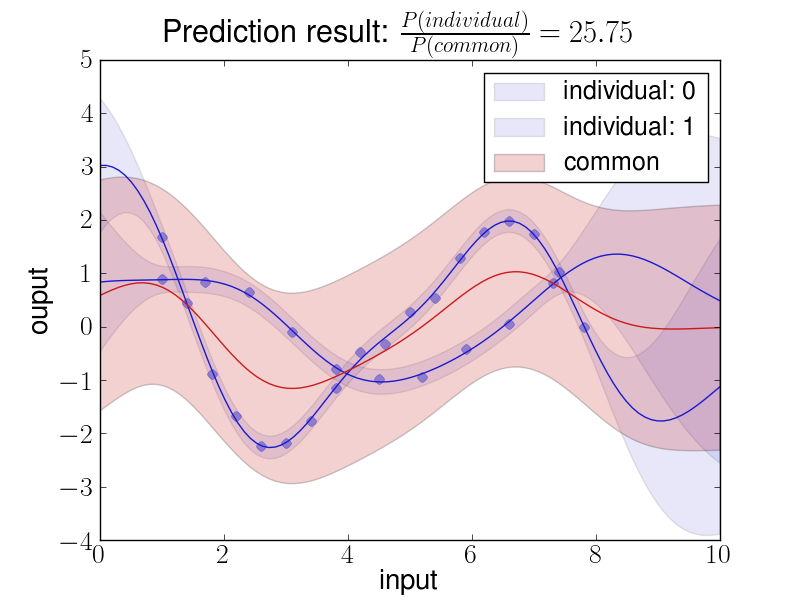
\includegraphics[height=8cm]{plotGPTwoSampleDifferential.png}

\textbf{Non-Differential Groups:}

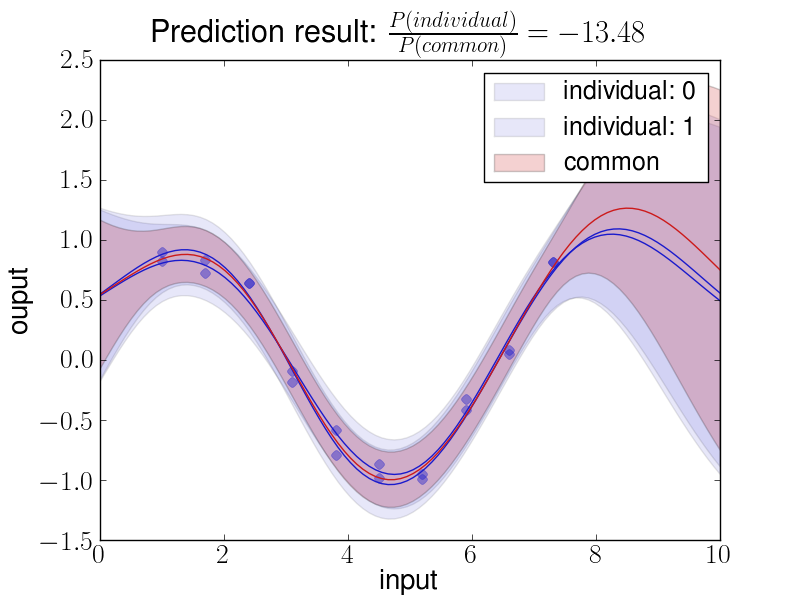
\includegraphics[height=8cm]{plotGPTwoSampleSame.png}
\begin{description}
\item[{Returns:}] \leavevmode
Proper rectangles for use in pylab.legend().

\end{description}

\end{fulllineitems}


\#  .. automodule:: gptwosample.plot.interval
\#    :members:
\phantomsection\label{data:module-gptwosample.data}\index{gptwosample.data (module)}

\chapter{Package for data handling}
\label{data:package-for-data-handling}\label{data::doc}
Use this Package for easiest way to handle the data for GPTwoSample.
\phantomsection\label{data:module-gptwosample.data.data_base}\index{gptwosample.data.data\_base (module)}

\section{Data Structure Module}
\label{data:data-structure-module}
This Module is for easy access to data structures gptwosample works with.

Created on Mar 18, 2011

@author: Max Zwiessele
\index{DataStructureError}

\begin{fulllineitems}
\phantomsection\label{data:gptwosample.data.data_base.DataStructureError}\pysiglinewithargsret{\strong{exception }\code{gptwosample.data.data\_base.}\bfcode{DataStructureError}}{\emph{*args}, \emph{**kwargs}}{}
Bases: \code{exceptions.TypeError}

Thrown, if DataStructure given does not fit.
Training data training\_data has following structure:

\begin{Verbatim}[commandchars=\\\{\}]
\PYGZob{}input\_id : \PYGZob{}'group 1':[double] ... 'group n':[double]\PYGZcb{},
 output\_id : \PYGZob{}'group 1':[double] ... 'group n':[double]\PYGZcb{}\PYGZcb{}
\end{Verbatim}

\end{fulllineitems}

\index{get\_model\_structure() (in module gptwosample.data.data\_base)}

\begin{fulllineitems}
\phantomsection\label{data:gptwosample.data.data_base.get_model_structure}\pysiglinewithargsret{\code{gptwosample.data.data\_base.}\bfcode{get\_model\_structure}}{\emph{individual=None}, \emph{common=None}}{}
Returns the valid structure for model dictionaries, used in gptwosample.
Make sure to use this method if you want to use the model structure in this package!

\end{fulllineitems}

\index{get\_training\_data\_structure() (in module gptwosample.data.data\_base)}

\begin{fulllineitems}
\phantomsection\label{data:gptwosample.data.data_base.get_training_data_structure}\pysiglinewithargsret{\code{gptwosample.data.data\_base.}\bfcode{get\_training\_data\_structure}}{\emph{x1}, \emph{x2}, \emph{y1}, \emph{y2}}{}
Get the structure for training data, given two inputs x1 and x2
with corresponding outputs y1 and y2. Make sure, that replicates have
to be tiled one after the other for proper resampling of data!

\end{fulllineitems}

\index{has\_model\_structure() (in module gptwosample.data.data\_base)}

\begin{fulllineitems}
\phantomsection\label{data:gptwosample.data.data_base.has_model_structure}\pysiglinewithargsret{\code{gptwosample.data.data\_base.}\bfcode{has\_model\_structure}}{\emph{structure}}{}
Returns the valid structure for model dictionaries, used in gptwosample.
Make sure to use this method if you want to use the model structure in this package!

\end{fulllineitems}

\phantomsection\label{data:module-gptwosample.data.dataIO}\index{gptwosample.data.dataIO (module)}

\section{Data IO tool}
\label{data:data-io-tool}
For convienent usage this module provides IO operations for data

Created on Jun 9, 2011

@author: Max Zwiessele, Oliver Stegle
\index{get\_data\_from\_csv() (in module gptwosample.data.dataIO)}

\begin{fulllineitems}
\phantomsection\label{data:gptwosample.data.dataIO.get_data_from_csv}\pysiglinewithargsret{\code{gptwosample.data.dataIO.}\bfcode{get\_data\_from\_csv}}{\emph{path\_to\_file}, \emph{delimiter='}, \emph{`}, \emph{count=-1}, \emph{verbose=True}, \emph{message='Reading File'}}{}
Return data from csv file with delimiter delimiter in form of a dictionary.
Missing Values are all values x which cannot be converted float(x)

The file format has to fullfill following formation:

\begin{tabulary}{\linewidth}{|L|L|L|L|}
\hline
\textbf{
\emph{arbitrary}
} & \textbf{
x1
} & \textbf{
...
} & \textbf{
xl
}\\\hline

Gene Name 1
 & 
y1 replicate 1
 & 
...
 & 
yl replicate 1
\\\hline

...
 & 
...
 & 
...
 & 
...
\\\hline

Gene Name 1
 & 
y1 replicate k1
 & 
...
 & 
yl replicate k1
\\\hline

...
 &  &  & \\\hline

Gene Name n
 & 
y1 replicate 1
 & 
...
 & 
yl replicate 1
\\\hline

...
 & 
...
 & 
...
 & 
...
\\\hline

Gene Name n
 & 
y1 replicate kn
 & 
...
 & 
yl replicate kn
\\\hline
\end{tabulary}


Returns: \{``input'':{[}x1,...,xl{]}, ``Gene Name 1'':{[}{[}y1 replicate 1, ... yl replicate 1{]}, ... ,{[}y1 replicate k, ..., yl replikate k{]}{]}\}

\end{fulllineitems}

\index{write\_data\_to\_csv() (in module gptwosample.data.dataIO)}

\begin{fulllineitems}
\phantomsection\label{data:gptwosample.data.dataIO.write_data_to_csv}\pysiglinewithargsret{\code{gptwosample.data.dataIO.}\bfcode{write\_data\_to\_csv}}{\emph{data}, \emph{path\_to\_file}, \emph{header='GPTwoSample'}, \emph{delimiter='}, \emph{`}}{}
Write given data in training\_data\_structure (see {\hyperref[data:module-gptwosample.data.data_base]{\code{gptwosample.data.data\_base}}} for details)
into file for path\_to\_file.

\textbf{Parameters:}
\begin{description}
\item[{data}] \leavevmode{[}dict{]}
data to write in training\_data\_structure

\item[{path\_to\_file}] \leavevmode{[}String{]}
The path to the file to write to

\item[{header}] \leavevmode{[}String{]}
Name of the table

\item[{delimiter}] \leavevmode{[}character{]}
delimiter for the csv file

\end{description}

\end{fulllineitems}



\chapter{Indices and tables}
\label{index:indices-and-tables}\begin{itemize}
\item {} 
\emph{genindex}

\item {} 
\emph{modindex}

\item {} 
\emph{search}

\end{itemize}


\renewcommand{\indexname}{Python Module Index}
\begin{theindex}
\def\bigletter#1{{\Large\sffamily#1}\nopagebreak\vspace{1mm}}
\bigletter{g}
\item {\texttt{gptwosample}}, \pageref{base:module-gptwosample}
\item {\texttt{gptwosample.data}}, \pageref{data:module-gptwosample.data}
\item {\texttt{gptwosample.data.data\_base}}, \pageref{data:module-gptwosample.data.data_base}
\item {\texttt{gptwosample.data.dataIO}}, \pageref{data:module-gptwosample.data.dataIO}
\item {\texttt{gptwosample.plot}}, \pageref{plot:module-gptwosample.plot}
\item {\texttt{gptwosample.plot.plot\_basic}}, \pageref{plot:module-gptwosample.plot.plot_basic}
\end{theindex}

\renewcommand{\indexname}{Index}
\printindex
\end{document}
